\chapter{스핀, 측정, 그리고 2차원 상태 공간}

\lectureoverview{스핀은 방향성을 띠지만, 스핀의 각 성분을 측정하면 결과는 \(+1\) 또는 \(-1\)뿐이다. 먼저 이 조작적 수수께끼를 정식화한 다음, 양립할 수 없는 측정에서는 왜 보통의 집합 논리가 성립하지 않는지 살펴본다. 적절한 언어는 2차원 복소 벡터 공간이다. 확률은 진폭에서 나오고, 구별 가능한 대안은 서로 직교하며, 위--아래, 오른쪽--왼쪽, 안쪽--바깥쪽 기저는 상태 벡터를 보통의 화살표로 바꾸지 않으면서 세 공간 방향을 나타낸다.}

\section{큐비트에서 스핀으로}

앞서 큐비트로 도입한 두 상태 계를 이제 \emph{스핀}이라고 부르겠다. 이름을 바꾸면 논의에 공간 방향이 들어오지만, \emph{벡터}라는 말에 혼동이 생길 위험도 있다. 서로 다른 두 대상을 구별해야 한다.

\begin{definition}
\emph{삼차원 벡터}는 3차원 공간에 놓인 보통의 실수 벡터다. 수식어 없이 \emph{벡터}라고 하면 양자역학에서 쓰는 복소 상태 공간처럼 추상적인 벡터 공간의 원소를 뜻한다.
\end{definition}

스핀은 보통 공간의 한 축을 기준으로 준비할 수 있다. 그러나 그 상태는 추상 벡터로 표현된다. 이 두 진술의 관계는 우리가 알아내야 할 내용 중 하나이며, 그림만 보고 미리 가정할 수는 없다.

\section{측정 장치를 빼놓을 수 없는 이유}

고전역학에서는 이상적인 관찰자가 계를 가능한 한 적게 교란하면서 계에 대해 알아낼 수 있다고 생각하기 쉽다. 예를 들어 거시적 물체를 본다고 하자. 물체를 비추고, 렌즈로 반사광을 모아 상을 확대한다. 빛은 힘을 가하지만, 고전적인 이상화에서는 빛의 세기를 줄이는 동시에 확대율을 높일 수 있다. 측정이라는 생각을 포기하지 않고도 교란을 임의로 작게 만들 수 있다.

이 극한 절차는 양자역학에서는 성립하지 않는다. 측정 장치를 개선하고 차폐하고 보정할 수는 있지만, 일반적으로 측정을 정보를 주면서도 임의로 비침습적이게 만들 수는 없다. 계의 어떤 것이 변한다. 그렇다고 모든 측정이 모든 성질을 파괴한다거나 결과를 재현할 수 없다는 뜻은 아니다. 측정 장치는 물리적으로 던지는 질문의 일부이며, 측정 후의 상태를 무시할 수 없다는 뜻이다.

일단 측정 장치를 두 가지 특성을 가진 블랙박스로 생각하자. 공간에서 방향을 정할 수 있고, 표시창에는 \(+1\) 또는 \(-1\)가 기록된다. 칠판에 그린 작은 화살표는 준비된 스핀을 표시하는 편리한 표식이다.

\begin{figure}[htbp]
\centering
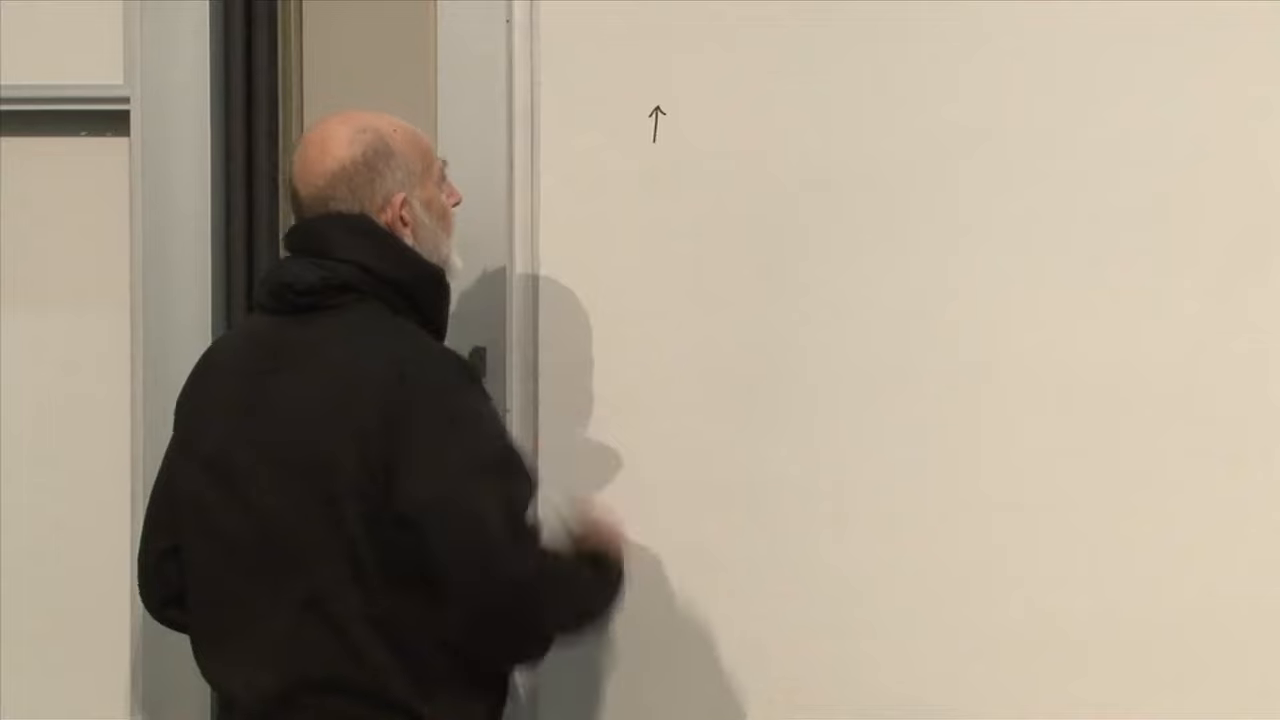
\includegraphics[width=0.64\textwidth]{lecture_02_figure_02.png}
\caption{한 축을 따라 준비된 스핀을 나타내는 잠정적인 첫 표식. 화살표는 준비 방향을 표시할 뿐, 아직 상태의 고전적 모형은 아니다.}
\lectureframe{00:05:15}
\end{figure}

축을 정해 \(z\)은 칠판 위쪽을, \(x\)는 오른쪽을, \(y\)는 칠판 바깥쪽을 가리키게 하자. 측정 장치를 단위 방향 \(\hat m\)에 맞추면 결과는 다음과 같다.
\begin{equation}
\sigma_{\hat m}=\pm1.
\end{equation}
특히,
\[
\sigma_z=\pm1,\qquad \sigma_x=\pm1,\qquad \sigma_y=\pm1.
\]
이 단계에서 \emph{성분}이라는 말은 조작적으로 정의된다. \(\sigma_z\)는 장치가 \(z\) 방향을 향할 때 그 장치가 보고하는 값이다. 아직 숨겨진 고전적 화살표의 \(z\) 성분을 뜻하는 것은 아니다.

\subsection{반복 가능성과 교란}

\(z\) 측정에서 \(+1\)가 나왔다고 하자. 그 사이에 다른 조작이 없으면 두 번째 \(z\) 측정에서도 다시 \(+1\)가 나오며, 이후 반복 측정에서도 마찬가지다. 첫 측정은 바로 그 질문에 확정된 답이 나오도록 상태를 준비했다.

\begin{classroomqa}
\audiencequestion{양자 측정이 스핀을 교란한다면, 바로 반복 측정했을 때는 왜 같은 결과가 나오나요?}
\lecturerresponse{교란이 무차별적으로 일어나는 것은 아니다. \(\sigma_z\)를 측정하면 이후의 \(x\) 또는 \(y\) 측정 결과는 달라질 수 있지만, 방금 측정한 \(\sigma_z\) 값은 재현 가능하게 남을 수 있다. 유용한 실험에는 바로 이런 제한된 안정성이 필요하다.}
\end{classroomqa}

이제 장치를 \(180^\circ\) 돌려 보자. 위쪽을 향한 방향에서 \(+1\)를 낸 스핀은 방향을 뒤집으면 \(-1\)을 낸다. 장치를 다시 똑바로 세우면 결과는 \(+1\)이다. 따라서 방향이 중요하다. 온도계는 거꾸로 돌렸다고 온도의 음수를 표시하지 않지만, 스핀 분석기는 방향에 관한 질문을 하기 때문에 다르게 작동한다.

\begin{figure}[htbp]
\centering
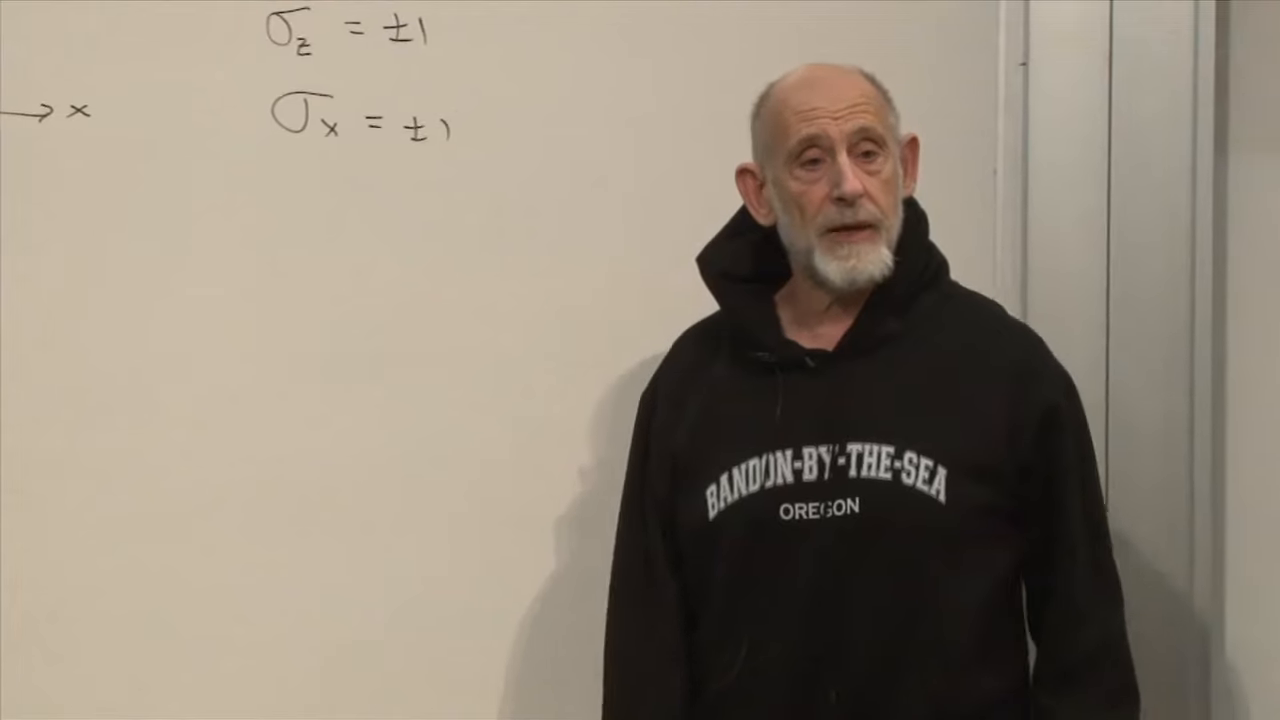
\includegraphics[width=0.72\textwidth]{lecture_02_figure_03.png}
\caption{칠판에는 두 값 \(\sigma_z=\pm1\)와 \(\sigma_x=\pm1\), 그리고 \(x\)축의 방향 표식이 함께 적혀 있다.}
\lectureframe{00:12:46}
\end{figure}

고전적인 단위 벡터와의 차이는 분명하다. 고전적 성분은 \(-1\)과 \(+1\) 사이에서 연속적으로 변한다. \(x\)축에 수직인 단위 벡터의 \(x\) 성분은 0이다. 반면 \(x\) 방향을 향한 스핀 분석기는 0을 표시하지 않는다. 스핀이 \(z\) 방향으로 준비되었더라도 \(+1\) 또는 \(-1\)을 표시한다.

\section{개별 결과와 벡터처럼 변하는 평균}

\(\sigma_z=+1\)를 얻어 스핀을 준비한 다음 \(\sigma_x\)를 측정하자. 동일하게 준비한 시행의 절반에서는 \(+1\)가, 나머지 절반에서는 \(-1\)가 나온다. 따라서
\begin{equation}
\langle \sigma_x\rangle=0.
\end{equation}
같은 준비에서
\begin{equation}
\langle \sigma_y\rangle=0.
\end{equation}
도 성립한다. 반대로 \(\sigma_x=+1\)인 스핀을 준비하면 이어지는 \(z\) 또는 \(y\) 측정에서 두 결과가 같은 확률로 나온다.

그 진술에는 서로 다른 두 실험이 담겨 있다. 첫 \(\sigma_x\) 측정에서 \(x\) 결과를 얻은 뒤 \emph{같은} 스핀을 반복 측정해도 그 결과를 확인할 뿐이다. 반--반 통계를 얻으려면 같은 \(z\) 상태로 준비한 스핀이 많이 필요하거나, 한 스핀을 각 \(x\) 측정 전에 같은 상태로 다시 준비해야 한다.

\begin{classroomqa}
\audiencequestion{스핀을 일부러 준비하지 않고 측정 장치에 넣으면 어떻게 되나요?}
\lecturerresponse{결과는 여전히 \(+1\) 또는 \(-1\)이지만, 각 결과의 확률은 스핀이 실제로 어떤 상태에 있는지에 따라 달라진다. 준비란 반복 시행을 서로 비교할 수 있게 만드는 통제된 절차다. 두 측정 사이에 알려지지 않은 조작이 일어나면 결과가 반복된다고 보장할 수 없다. 아무 일도 일어나지 않으면 같은 성분의 측정 결과는 재현 가능하다.}
\end{classroomqa}

\subsection{임의의 두 방향}

\(\hat n\) 방향의 분석기에 통과시켜 \(+1\)을 얻음으로써 스핀을 단위 방향 \(\hat n\)을 따라 준비한다. 그런 다음 다른 단위 방향 \(\hat m\)을 따라 측정한다. 각 시행에서 여전히 \(\pm1\)만 나오지만, 동일하게 준비한 시행들의 평균은
\begin{equation}
\boxed{\langle\sigma_{\hat m}\rangle=\hat n\cdot\hat m
=\cos\theta_{nm}.}
\label{eq:spin-average}
\end{equation}
칠판에는 더 짧은 표기인 \(\langle\sigma_m\rangle=n\cdot m\)를 사용한다:

\begin{figure}[htbp]
\centering
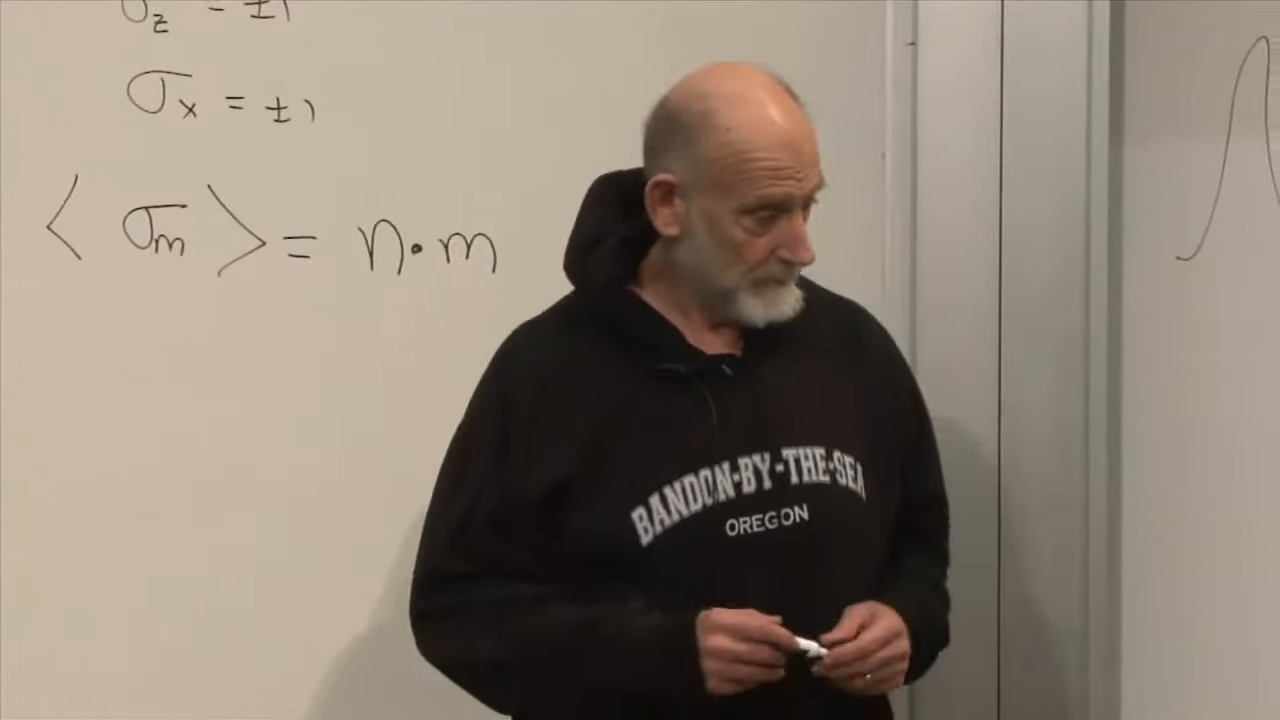
\includegraphics[width=0.74\textwidth]{lecture_02_figure_04.png}
\caption{벡터처럼 변하는 법칙은 개별 \(\pm1\) 결과가 아니라 앙상블 평균에 적용된다.}
\lectureframe{00:23:22}
\end{figure}

식~\eqref{eq:spin-average}에는 앞서 본 경우들이 포함된다. \(\hat m=\hat n\)이면 평균은 \(+1\)이다. 어떤 결과도 \(+1\)를 넘을 수 없으므로 모든 시행에서 \(+1\)가 나온다. \(\hat m=-\hat n\)이면 모든 시행에서 \(-1\)가 나온다. 서로 수직인 축에서는 평균이 0이고 두 결과의 빈도가 같다.

\(p_+\)와 \(p_-\)를 두 가능한 결과가 나올 확률이라고 하면
\[
p_++p_-=1,\qquad p_+-p_-=\hat n\cdot\hat m.
\]
따라서
\begin{equation}
p_\pm=\frac{1\pm\hat n\cdot\hat m}{2}.
\label{eq:direction-probabilities}
\end{equation}
\editorialnote{강의에서는 두 결과와 그 평균을 제시한다. 식~\eqref{eq:direction-probabilities}은 이 두 사실에서 직접 따라오는 대수적 결과다.}

\begin{classroomqa}
\audiencequestion{꺾쇠괄호 안의 양은 \emph{기댓값}인가요, 아니면 보통의 평균인가요?}
\lecturerresponse{이는 여러 번 반복해 기록한 결과의 평균이다. \emph{기댓값}은 표준 용어지만, 여기서 별도의 평균 방식을 뜻하지는 않는다. 장치는 \(+1\)과 \(-1\)으로 이루어진 목록을 만들며, 괄호는 큰 앙상블 극한에서 그 목록의 산술평균을 나타낸다.}
\end{classroomqa}

\begin{classroomqa}
\audiencequestion{평균 법칙을 알기 전부터 화살표 \(\hat n\)에는 기하학적 의미가 있었나요?}
\lecturerresponse{처음에는 준비 장치의 방향을 나타내는 표식이었다. 반전 실험과 평균이 \(\hat n\cdot\hat m\)에 따라 달라진다는 사실이 그 표식에 조작적 기하학의 의미를 부여한다. 성분의 의미는 장치가 정한다. 개별 결과만으로는 고전적 투영값을 얻을 수 없다.}
\end{classroomqa}

이것이 방향에 관한 그림과 이산적인 데이터가 처음으로 조화를 이루는 방식이다. 개별 스핀은 성분이 연속적으로 변하는 고전적 화살표처럼 행동하지 않는다. 그럼에도 동일하게 준비한 여러 스핀의 통계는 단위 삼차원 벡터의 성분과 정확히 같은 방식으로 변환된다.

\section{집합으로 나타내는 고전 명제}

양자 상태 공간을 구성하기 전에 고전계에서는 논리가 어떻게 작동하는지 생각해 보자. 가능한 상태들의 집합을 \(\Omega\)라 하자. 명제 \(A\)는 \(A\)가 참인 상태들의 부분집합으로 나타낸다.

6면체 주사위의 경우,
\[
A=\{2,4,6\}
\]
는 \emph{결과가 짝수다}를 나타낼 수 있고,
\[
B=\{4,5,6\}
\]
는 \emph{결과가 3보다 크다}를 나타낼 수 있다. 논리 연산은 집합 연산이 된다.
\begin{equation}
\neg A=A^c,\qquad
A\land B=A\cap B,\qquad
A\lor B=A\cup B.
\label{eq:classical-logic}
\end{equation}
여기서 \(\lor\)는 포함적 OR다. \(A\lor B\)는 \(A\)가 참이거나 \(B\)가 참이거나 둘 다 참일 때 참이다. 일상에서 쓰는 \emph{둘 중 하나\(A\) 또는 \(B\)둘 중 다른 하나지만 둘 다는 아님}이라는 배타적 의미가 아니다.

\begin{classroomqa}
\audiencequestion{스핀 측정에는 결과가 두 개뿐이지만 준비 방향은 연속적으로 달라질 수 있네요. 상태 집합은 유한한가요, 연속적인가요?}
\lecturerresponse{선택한 각 분석기에는 판독값이 두 개뿐이지만, 가능한 준비 방향의 집합은 연속적이다. 그래서 검출기 표시값의 수만 세어서는 상태 공간을 기술하기에 충분하지 않다.}
\end{classroomqa}

고전적 부분집합에서는 교집합과 합집합을 취할 때 명제의 순서가 중요하지 않다.
\[
A\cap B=B\cap A,\qquad A\cup B=B\cup A.
\]
따라서 고전적인 복합 명제를 실험적으로 검증하는 절차는 논리에 순서를 도입하지 않고 이상화할 수 있다.

\section{순서에 따라 달라지는 OR 검정}

다음 양자 명제들을 생각하자.
\begin{equation}
A:\sigma_z=+1,\qquad B:\sigma_x=+1.
\end{equation}
각 명제에는 명확한 검정 방법이 있다. 장치를 \(z\) 방향으로 맞추면 \(A\)를 검정하고, \(x\) 방향으로 맞추면 \(B\)를 검정한다. 한 명제를 먼저 검정하고 그것이 거짓이면 다른 명제를 검정해 \(A\lor B\)를 확인하려 할 때 문제가 드러난다.

보이지 않는 준비자가 \(z\) 방향으로 스핀을 준비했다고 하자. 먼저 \(A\)를 검정하면 결과는 확실히 \(+1\)이고, OR 검정은 \emph{참}으로 끝난다.

순서를 바꾸어 보자. 먼저 \(B\)를 검사하면
\[
P(B)=\frac12,\qquad P(\neg B)=\frac12.
\]
\(B\)가 거짓이어도 \(x\) 측정은 확정된 \(x\) 상태를 준비한다. 이 상태에서 \(A\)를 검사하면
\[
P(A\mid \neg B)=\frac12,\qquad
P(\neg A\mid \neg B)=\frac12.
\]
따라서 순서를 바꾼 절차에서 두 명제가 모두 거짓으로 판정될 확률은
\begin{equation}
P(\neg B\ \text{then}\ \neg A)
=\frac12\cdot\frac12=\frac14.
\end{equation}
이다. 한 순서에서는 OR가 항상 참으로 판정되지만, 다른 순서에서는 시행의 사분의 일에서 거짓으로 판정된다.

\begin{classroomqa}
\audiencequestion{이 모순은 몰래 준비된 상태에 대한 우리의 불완전한 지식에서 비롯된 것뿐인가요?}
\lecturerresponse{아니다. 비교를 분명히 하려고 숨겨진 준비 상태를 택했을 뿐이다. 첫 \(x\) 측정은 물리적으로 \(x\) 상태를 준비하므로, 뒤이은 \(z\) 검정은 변한 상태에서 이루어진다. 처음 준비에 관해 관찰자에게 더 많은 정보를 주더라도 그 개입을 되돌릴 수는 없다.}
\end{classroomqa}

\begin{classroomqa}
\audiencequestion{이런 순차 규칙 대신 더 복잡한 질문의 계층을 이용해 OR을 검정할 수 있나요?}
\lecturerresponse{물론 서로 다른 실험 절차를 정의할 수는 있지만, 그러면 서로 다른 양자 측정이 된다. 장치와 무관하게 참인지 여부만 드러나는 절차 독립적인 부분집합 \(A\cup B\)는 존재하지 않는다. 순서 의존성은 고전적 집합 논리가 이 명제들에 본래 적용되는 논리가 아니라는 경고다.}
\end{classroomqa}

나중에는 사영 연산자로 명제를 나타낼 것이다. 간결한 대수적 경고는 다음과 같다.
\begin{equation}
P_A P_B\ne P_B P_A.
\end{equation}
아직 연산자 이론을 더 끌어올 필요는 없다. 중요한 점은 양립할 수 없는 검정들이 가환하지 않으며, 그 복합 명제를 보통의 집합 합집합처럼 다룰 수 없다는 것이다.

\begin{classroomqa}
\audiencequestion{검정 선택이 시간상 과거에 영향을 미치는 두 입자 실험을 구성할 수 있나요?}
\lecturerresponse{그 질문에 답하려면 아직 다루지 않은 수학적 도구가 필요하다. 한 스핀의 순차 측정만으로는 과거 방향 인과성에 관한 결론을 내릴 수 없으므로, 추측으로 답하지 않고 문제를 열어 둔다.}
\end{classroomqa}

\section{선형 상태 공간}

집합에는 원소가 들어 있지만, 두 원소를 더해 세 번째 원소를 얻는 자연스러운 방법은 일반적으로 없다. 선형 벡터 공간에는 더 많은 구조가 있다. \(\ket{A}\)와 \(\ket{B}\)가 벡터이고 \(\alpha,\beta\in\mathbb C\)이면
\begin{equation}
\alpha\ket{A}+\beta\ket{B}
\end{equation}
도 같은 공간의 벡터다. 양자 상태는 이러한 복소 선형 공간에서 나타낸다.

각 켓 \(\ket{A}\)에는 대응하는 쌍대 브라 \(\bra{A}\)가 있다. 브라와 켓을 짝지으면 복소수인 내적을 얻는다. 내적은 켤레 대칭을 만족한다.
\begin{equation}
\braket{A}{B}=\braket{B}{A}^{*}.
\label{eq:conjugate-symmetry}
\end{equation}

\begin{figure}[htbp]
\centering
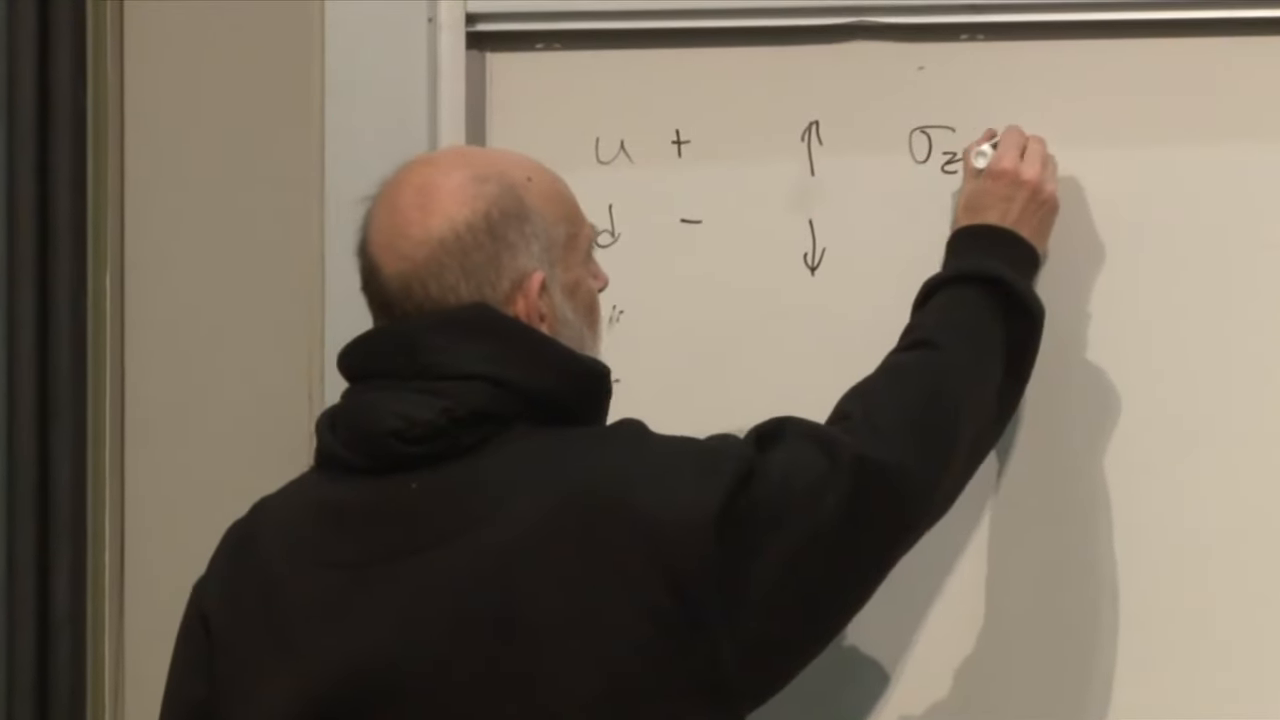
\includegraphics[width=0.78\textwidth]{lecture_02_figure_05.png}
\caption{칠판에는 선형 결합과 내적에서 켤레를 취할 때 순서가 뒤바뀌는 성질이 요약되어 있다.}
\lectureframe{00:46:53}
\end{figure}

벡터의 길이의 제곱은 다음과 같다.
\begin{equation}
\|\ket{A}\|^2=\braket{A}{A}.
\end{equation}
식~\eqref{eq:conjugate-symmetry}에 따르면 이 값은 자기 자신의 복소켤레와 같으므로 실수다. 내적의 공리상 이 값은 음이 아니기도 하다. 두 벡터가 직교한다는 것은 다음을 만족한다는 뜻이다.
\begin{equation}
\braket{A}{B}=0.
\end{equation}
공간의 차원은 서로 직교하는 영벡터가 아닌 방향을 선택할 수 있는 최대 개수다.

\begin{classroomqa}
\audiencequestion{모든 기저는 서로 직교하는 벡터로 이루어져야 하나요?}
\lecturerresponse{아니다. 기저가 되려면 선형 독립이고 공간을 생성하기만 하면 된다. 직교 기저에서는 계수와 확률을 쉽게 구할 수 있어 특히 편리하다. 2차원에서는 평행하지 않은 두 벡터가 내적이 0이 아니더라도 기저를 이룰 수 있다.}
\end{classroomqa}

\section{2차원 스핀 공간}

스핀 하나의 상태 공간은 2차원 복소 벡터 공간이라고 가정한다.
\begin{equation}
\mathcal H_{\mathrm{spin}}\cong\mathbb C^2.
\end{equation}
가능한 상태 벡터는 연속적으로 많지만, 어느 상태든 나타내는 데 필요한 선형 독립 기저 벡터는 두 개뿐이다.

\(z\) 방향으로 정렬된 장치가 준비한 상태부터 살펴보자:
\begin{align}
\ket{u}&\longleftrightarrow \sigma_z=+1,\\
\ket{d}&\longleftrightarrow \sigma_z=-1.
\end{align}
문자 \(u,d\), 부호 \(+,-\), 화살표 \(\uparrow,\downarrow\)는 같은 두 준비 상태를 나타내는 서로 다른 표기다. \(z\) 측정으로 두 상태를 확실하게 구별할 수 있으므로, 상태 벡터는 서로 직교한다:
\begin{equation}
\braket{u}{d}=0.
\end{equation}
상태 벡터의 길이를 단위 길이로 정하면
\[
\braket{u}{u}=\braket{d}{d}=1.
\]

그러면 모든 스핀 상태는 다음과 같이 쓸 수 있다.
\begin{equation}
\ket{A}=\alpha_u\ket{u}+\alpha_d\ket{d},
\qquad \alpha_u,\alpha_d\in\mathbb C.
\label{eq:general-spin-state}
\end{equation}
확률 규칙은 다음과 같다.
\begin{equation}
P(u|A)=|\alpha_u|^2,\qquad
P(d|A)=|\alpha_d|^2.
\label{eq:born-z}
\end{equation}
두 결과 중 하나는 반드시 나와야 하므로
\begin{equation}
|\alpha_u|^2+|\alpha_d|^2=1.
\label{eq:normalization}
\end{equation}

\begin{figure}[htbp]
\centering
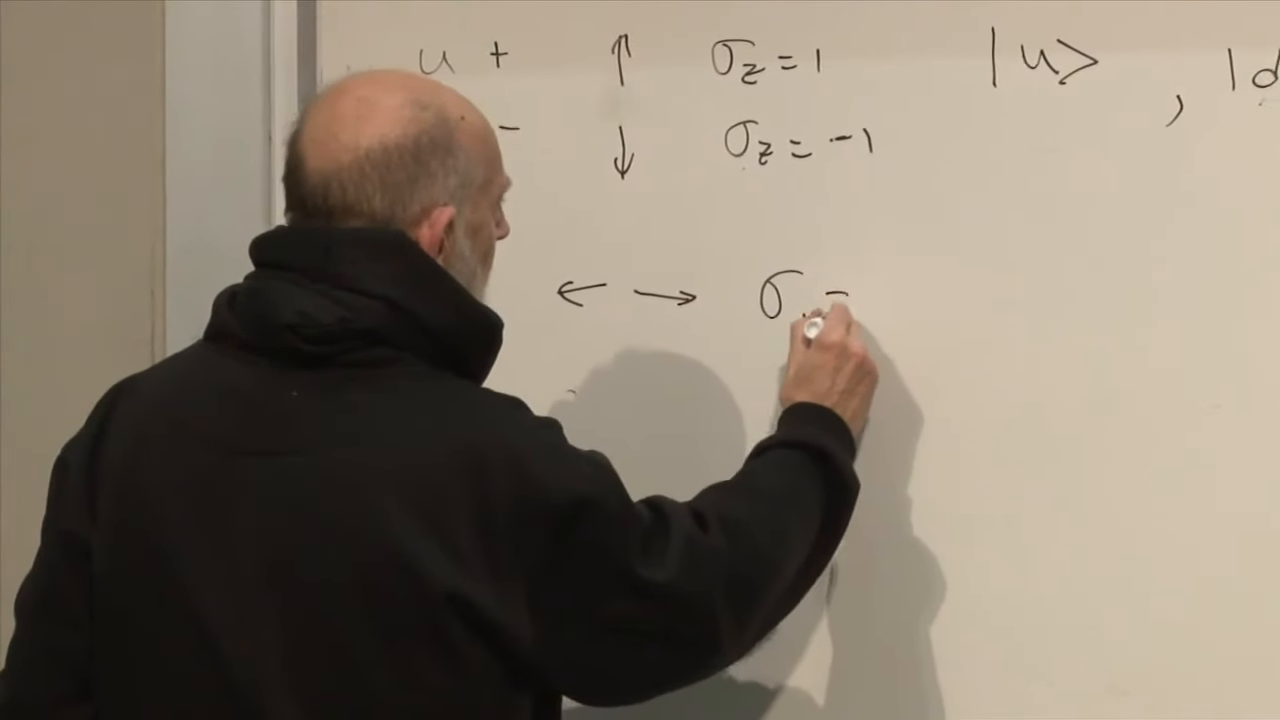
\includegraphics[width=0.78\textwidth]{lecture_02_figure_06.png}
\caption{일반적인 위--아래 전개, 두 결과 확률의 합, 그리고 이에 동등한 단위 노름 조건.}
\lectureframe{01:03:38}
\end{figure}

단위 정규화와의 동등성은 바로 다음과 같이 확인된다.
\begin{align}
\braket{A}{A}
&=(\alpha_u^*\bra{u}+\alpha_d^*\bra{d})
  (\alpha_u\ket{u}+\alpha_d\ket{d})\\
&=|\alpha_u|^2\braket{u}{u}
 +\alpha_u^*\alpha_d\braket{u}{d}\\
&\quad +\alpha_d^*\alpha_u\braket{d}{u}
 +|\alpha_d|^2\braket{d}{d}\\
&=|\alpha_u|^2+|\alpha_d|^2=1.
\end{align}
따라서 물리적인 순수 상태는 정규화된 벡터로 나타낸다.

\begin{classroomqa}
\audiencequestion{이 진술들은 유도된 것인가요, 아니면 공준인가요?}
\lecturerresponse{이 단계에서는 실험에 맞춰 세운 규칙이다. 2차원 공간, 확률 규칙, 직교성의 해석을 경험적 직관을 바탕으로 도입하고 있다. 이 규칙들이 서로 일관되는지는 지금 확인할 수 있다. 상태와 관측량의 체계적인 관계는 다음에 다룬다.}
\end{classroomqa}

\subsection{구별 가능성을 나타내는 직교성}

직교성의 물리적 의미는 서로 수직인 화살표 그림보다 더 유용하다.

\begin{quote}
한 번의 측정으로 확실히 구별할 수 있는 상태는 직교 벡터로 나타낸다.
\end{quote}

위와 아래는 이 기준을 만족한다. 상태가 위쪽이면 \(z\) 장치는 아래쪽 결과를 내지 않으며, 그 반대도 마찬가지다. 내적이 영이 아니면 한 상태에서 다른 상태에 대응하는 결과가 나올 수 있음을 뜻한다.

\section{오른쪽--왼쪽 기저}

\(\ket{r}\)와 \(\ket{l}\)를 \(x\) 스핀이 확정된 상태라고 하자.
\[
\ket{r}\longleftrightarrow\sigma_x=+1,\qquad
\ket{l}\longleftrightarrow\sigma_x=-1.
\]
공간이 2차원이므로 각각을 \(\ket{u}\)와 \(\ket{d}\)의 선형 결합으로 쓸 수 있다. 오른쪽 방향으로 준비한 스핀은 위와 아래 결과를 같은 확률로 내므로 두 계수의 크기는 같아야 한다. 가장 간단한 위상 규약을 택하면 다음과 같다.
\begin{equation}
\ket{r}=\frac{1}{\sqrt2}\bigl(\ket{u}+\ket{d}\bigr).
\label{eq:right-state}
\end{equation}
\(x\) 장치로 오른쪽과 왼쪽 상태를 확실히 구별할 수 있으므로 왼쪽 상태는 오른쪽 상태와 직교해야 한다. 편리한 선택은 다음과 같다.
\begin{equation}
\ket{l}=\frac{1}{\sqrt2}\bigl(\ket{u}-\ket{d}\bigr).
\label{eq:left-state}
\end{equation}
실제로
\begin{align}
\braket{l}{r}
&=\frac12(\bra{u}-\bra{d})(\ket{u}+\ket{d})\\
&=\frac12(1-1)=0.
\end{align}

\begin{figure}[htbp]
\centering
\includegraphics[width=0.82\textwidth]{lecture_02_figure_07.png}
\caption{완성된 오른쪽--왼쪽 구성. 위--아래 성분의 크기는 같고 상대 부호는 반대이며 내적은 0이다.}
\lectureframe{01:12:15}
\end{figure}

\(\ket{l}\)의 전체 부호는 규약에 따른 것이다. \(\ket{l}\)를 \(-\ket{l}\)로 바꾸어도 확률은 달라지지 않는다. 식~\eqref{eq:right-state}과 식~\eqref{eq:left-state}을 더하고 빼면 역 기저 변환을 얻는다.
\begin{align}
\ket{u}&=\frac{1}{\sqrt2}\bigl(\ket{r}+\ket{l}\bigr),\\
\ket{d}&=\frac{1}{\sqrt2}\bigl(\ket{r}-\ket{l}\bigr).
\end{align}
이 대칭성은 중요하다. \(x\) 기저에서 시작해도 위 또는 아래 상태는 오른쪽과 왼쪽의 같은 가중치 중첩이다. 오른쪽 또는 왼쪽 상태가 위와 아래의 같은 가중치 중첩인 것과 마찬가지다.

\section{안쪽--바깥쪽 기저와 상대 위상}

측정 장치를 칠판에 수직인 \(y\) 방향으로 맞춘다. 다음과 같이 쓴다.
\[
\ket{i}\longleftrightarrow\sigma_y=+1,\qquad
\ket{o}\longleftrightarrow\sigma_y=-1,
\]
여기서 켓 표기 \(i\)는 \emph{안쪽}을 뜻하며, 켓을 곱하는 꾸밈없는 \(i\)는 계속 허수 단위를 나타낸다.

위와 아래가 나올 확률이 같으려면 계수의 크기가 같아야 한다. 입사 상태와 출사 상태가 직교하려면 두 상태의 내적이 영이 되도록 상대 위상이 정해져야 한다. 대칭적인 선택은 다음과 같다:
\begin{align}
\ket{i}&=\frac{1}{\sqrt2}\bigl(\ket{u}+i\ket{d}\bigr),\\
\ket{o}&=\frac{1}{\sqrt2}\bigl(\ket{u}-i\ket{d}\bigr).
\label{eq:in-out-states}
\end{align}
\((u,d)\) 기저에서 여섯 상태는 다음과 같다:
\begin{align}
\ket{u}&=\binom10,
&
\ket{d}&=\binom01,
\\
\ket{r}&=\frac1{\sqrt2}\binom11,
&
\ket{l}&=\frac1{\sqrt2}\binom1{-1},
\\
\ket{i}&=\frac1{\sqrt2}\binom1{i},
&
\ket{o}&=\frac1{\sqrt2}\binom1{-i}.
\end{align}

\begin{figure}[htbp]
\centering
\includegraphics[width=0.82\textwidth]{lecture_02_figure_08.png}
\caption{위--아래 기저에서 나타낸 여섯 열벡터. 아래 두 벡터는 상대 허수 위상의 부호만 다르다.}
\lectureframe{01:20:50}
\end{figure}

브라에서 복소켤레를 취하는 것은 직교성을 확인할 때 필수다.
\begin{align}
\braket{i}{o}
&=\frac12(\bra{u}-i\bra{d})(\ket{u}-i\ket{d})\\
&=\frac12\bigl(1+(-i)(-i)\bigr)=0.
\end{align}

\begin{classroomqa}
\audiencequestion{안쪽\(+i\)을 \emph{in}으로, 바깥쪽\emph{을 }out}으로 두면 공간 축의 오른손잡이 방향을 나타내게 되나요?\lecturerresponse{규약이 하나 들어갔으며, 파울리 행렬과 회전을 다루면 그 기하학적 의미가 더 분명해질 것이다. 지금은 두 상태가 서로 직교하고 다른 기저들과 대칭적인 관계를 이루어야 한다는 점이 중요하다. 표기를 맞바꾸거나 \(y\)축을 반대로 뒤집으면 규약은 바뀌지만 구성의 일관성은 달라지지 않는다.}
\end{classroomqa}

\subsection{오른쪽--왼쪽 기저에서 대칭성 확인하기}

안쪽 상태에
\[
\ket{u}=\frac{\ket{r}+\ket{l}}{\sqrt2},\qquad
\ket{d}=\frac{\ket{r}-\ket{l}}{\sqrt2}
\]
를 사용하면
\begin{align}
\ket{i}
&=\frac1{\sqrt2}
\left(
\frac{\ket{r}+\ket{l}}{\sqrt2}
+i\frac{\ket{r}-\ket{l}}{\sqrt2}
\right)\\
&=\frac{1+i}{2}\ket{r}
 +\frac{1-i}{2}\ket{l}.
\label{eq:in-in-rl}
\end{align}
두 계수 어느 쪽에도 \(1/\sqrt2\)가 겉으로 나타나지 않지만,
\begin{equation}
\left|\frac{1+i}{2}\right|^2
=\left|\frac{1-i}{2}\right|^2
=\frac12.
\end{equation}

\begin{figure}[htbp]
\centering
\includegraphics[width=0.82\textwidth]{lecture_02_figure_09.png}
\caption{안쪽 상태의 실제 기저 변환과 오른쪽--왼쪽 결과의 확률이 각각 \(1/2\)임을 확인한 결과.}
\lectureframe{01:29:10}
\end{figure}

따라서 세 기저 중 하나의 상태를 다른 두 기저 중 어느 하나로 측정하면 두 결과가 같은 확률로 나온다. \(z\), \(x\), \(y\) 기저는 서로 상호 불편 상태다.

\section{서로 특별한 기저 쌍이 세 개인 이유}

\begin{classroomqa}
\audiencequestion{이 세 쌍이 서로에게 그러하듯 이들과 대칭적인 네 번째 상태 쌍도 있을 수 있나요?}단일한 2상태 계에서는 불가능하다. 세 쌍의 상호 불편 기저를 정하면, 이들과 같은 균일한 겹침 관계를 가진 네 번째 쌍은 없다. 이런 공간 방향 표지가 세 개라는 사실은 보통 공간의 차원이 3이라는 점과 연결되어 있다. 복소 상태 공간 자체의 차원은 2인데도 그렇다.\lecturerresponse{
}
\end{classroomqa}

물리적 매개변수를 세어 보면 이 연결을 알 수 있다. 일반적인 열벡터
\[
\binom{\alpha_u}{\alpha_d}
\]
에는 복소수 두 개, 즉 실수 네 개가 들어 있다. 정규화 조건 하나가 이를 줄인다.
\[
|\alpha_u|^2+|\alpha_d|^2=1.
\]
두 성분에 공통 위상을 곱해도 측정 확률은 변하지 않는다.
\begin{equation}
\ket{A}\sim e^{i\chi}\ket{A}.
\label{eq:global-phase}
\end{equation}
이로써 실수 매개변수가 하나 더 줄어든다. 따라서
\begin{equation}
4-1-1=2
\end{equation}
물리적 실수 매개변수는 두 개 남는다. 이는 3차원 공간에서 방향을 정하는 데 필요한 각도의 수와 정확히 같다.

관계를 분명히 보여주는 편리한 대표는 다음과 같다.
\begin{equation}
\ket{\psi(\theta,\phi)}
=\cos\frac{\theta}{2}\,\ket{u}
+e^{i\phi}\sin\frac{\theta}{2}\,\ket{d}.
\label{eq:bloch-parameterization}
\end{equation}
\editorialnote{~\eqref{eq:bloch-parameterization}은 강의에서 확인한 두 매개변수 족의 표준 정규화 대표다. 매개변수 개수를 구체적으로 보여주려고 명시적인 반각 표현을 포함했다. 이 표현의 동역학적 및 회전 관련 해석은 이후 강의에서 다룬다.}

\begin{classroomqa}
\audiencequestion{전체 위상을 무시한다는 것을 수학적으로 정확히 어떻게 표현하나요?}
\lecturerresponse{원 \(\{e^{i\chi}\ket{\psi}\}\) 위의 정규화 벡터들은 모두 같은 물리적 상태를 나타낸다. 선언된 중복성으로 서로 연결된 점들을 하나의 물리적 점으로 취급하듯, 이 벡터들을 동등한 것으로 본다. 성분 사이의 상대 위상은 측정할 수 있다. 버리는 것은 벡터 전체에 곱해진 위상뿐이다.}
\end{classroomqa}

\begin{classroomqa}
\audiencequestion{정규화되지 않은 벡터나 성분에 음수가 있는 벡터도 계산에 나타날 수 있나요?}
\lecturerresponse{그렇습니다. 선형대수에서는 그런 벡터도 허용되며, 중간 단계의 벡터가 아직 준비된 물리적 상태를 나타낼 필요는 없습니다. 영벡터가 아닌 벡터는 마지막에 정규화할 수 있습니다. 음수 성분과 복소수 성분은 확률이 아니라 확률 진폭입니다. 확률은 상태를 정규화한 뒤 성분의 절댓값을 제곱해 얻습니다.}
\end{classroomqa}

\begin{classroomqa}
\audiencequestion{더 높은 차원의 공간이나 더 복잡한 스피너에서는 이 그림이 어떻게 되나요?}
\lecturerresponse{같은 선형 원리는 계속 적용되지만, 상태 공간 차원과 공간 회전, 관측 가능한 스핀 사이의 관계는 더 풍부해진다. 그 확장은 지금 다루는 2상태 구성의 범위를 벗어난다.}
\end{classroomqa}

\section{직교성은 공간적 수직이 아니다}

이제 \emph{직교}라는 말은 추상적이고 조작적인 의미를 갖는다. 보통 공간에 그린 두 화살표 사이의 각도와 혼동해서는 안 된다. 공간 방향으로 위와 아래는 서로 반대지만 상태 벡터 \(\ket{u}\)와 \(\ket{d}\)는 직교한다. 공간 방향으로 위와 오른쪽은 서로 수직이지만,
\begin{equation}
\braket{u}{r}=\frac1{\sqrt2}\ne0.
\end{equation}

\begin{classroomqa}
\audiencequestion{공간에서 서로 반대 방향인 상태는 직교하는데, 서로 수직인 방향의 상태는 왜 직교하지 않나요?}
\lecturerresponse{상태 공간에서의 중첩은 표기가 나타내는 유클리드 각도가 아니라 실험적으로 구별할 수 있는지를 나타냅니다. 위와 아래 상태는 단 한 차례의 \(z\) 측정으로 확실하게 구별할 수 있으므로 중첩이 영입니다. 위와 오른쪽 상태는 확실하게 구별할 수 없습니다. 오른쪽으로 준비한 스핀은 때때로 위쪽 결과를 내기 때문입니다. 따라서 두 상태 벡터는 서로 중첩됩니다.}
\end{classroomqa}

이 생각에 대응하는 고전 확률론의 유사 개념도 있다. 지지집합이 서로 겹치지 않는 두 확률분포는 완벽하게 구별할 수 있다. 관측 결과로 어느 분포가 사용되었는지 알 수 있다. 지지집합이 겹치는 분포는 표본 하나만으로 오류 없이 구별할 수 없다. 양자역학에서 직교성은 지지집합이 겹치지 않는 경우에 해당하고, 영이 아닌 내적은 어떤 결과가 어느 쪽 준비 상태에서든 나올 수 있음을 나타낸다.

\begin{classroomqa}
\audiencequestion{2차원 상태 공간을 위쪽 화살표와 오른쪽 화살표가 놓인 물리적 평면으로 시각화해야 하나요?}
\lecturerresponse{아니다. 표지 \(x,y,z\)는 보통 공간에서 측정 장치가 향하는 방향을 가리킨다. 켓은 고유한 내적을 갖는 복소 벡터 공간에 속한다. 매개변수 개수는 두 구조를 연결하지만, 두 그림을 점대점으로 동일시하면 공간적 수직성과 상태 공간의 직교성을 혼동하게 된다.}
\end{classroomqa}

\section{상태, 측정, 그리고 앞으로 다룰 내용}

지금까지는 관측 가능한 사실에 맞도록 벡터를 정하는 방식으로 구성해 왔다. 세 방향의 장치는 각각 정규화된 상태 두 개를 나타내며, 상태들 사이의 내적은 관측된 확률을 재현한다. 엄밀하게 다루려면 \(\sigma_z\) 같은 관측량이 상태에 어떻게 작용하는지, 그리고 가능한 결과가 왜 그 관측량의 고윳값인지도 설명해야 한다. 다음 단계에서 이를 살펴본다.

앞서 나온 논리 퍼즐을 이제 더 분명하게 표현할 수 있다. 명제는 부분공간이나 그 사영 연산자에 대응하며, 서로 양립할 수 없는 사영 연산자는 서로 가환하지 않는다. 순서에 따라 결과가 달라지는 OR 검사는 말장난에서 비롯된 역설이 아니었다. 그것은 비가환 구조가 처음 드러난 사례였다.

\begin{classroomqa}
\audiencequestion{상태가 보통 의미의 화살표가 아니라면, 세 표지 \(x,y,z\)와 평균 \(\langle\sigma_{\hat m}\rangle\)은 왜 그렇게 고전적으로 보이나요?}
\lecturerresponse{고전적인 벡터는 앙상블 평균에서 나타납니다. 스핀 하나에서는 이산적인 결과가 나오지만, 동일하게 준비한 스핀을 많이 측정하면 방향의 성분처럼 변환하는 평균값을 얻습니다. 큰 집합에서 평균값이 안정되면 거시적인 고전 거동이 나타납니다. 그렇다고 이를 거꾸로 해석해 개별 스핀마다 숨겨진 연속적인 값이 있다고 보아서는 안 됩니다.}
\end{classroomqa}

\begin{classroomqa}
\audiencequestion{공통 위상에 대한 중복성도 게이지 불변성의 한 예인가요?}
\lecturerresponse{이는 공통 위상에 대한 단순한 불변성이며, 더 넓은 게이지 개념을 예고합니다. 여기서 그 연관성을 발전시키면 현재의 구성 범위를 벗어나므로, 물리적으로 중요한 진술만 남기겠습니다. 공통 위상은 관측되지 않지만 상대 위상은 관측됩니다.}
\end{classroomqa}

마지막으로, 측정을 고전적 의미에서 스핀이 줄곧 지니고 있던 값을 그저 밝혀내는 과정으로 그려서는 안 된다. 측정은 기록된 결과에 대응하는 상태를 준비한다. 따라서 같은 측정을 곧바로 반복해도 모순이 없으며, 동일하게 준비한 스핀으로 이루어진 새로운 앙상블에서는 관련 진폭이 정하는 확률분포가 나타난다. 관측량을 연산자로 도입하면 이러한 상태 준비와 측정 결과의 수학적 기술이 명확해질 것이다.